\newpage
\section{Exercises: Sinusoidal Signals}

Hint: You can often write a Python program to verify your result if you are not sure if it is correct!

\begin{enumerate}

  % Exercise 1
  \item You may have heard somebody say that noise-cancelling headphones
        rely on playing an audio signal where each spectral component of the
        signal is perfectly ``out of phase'' with the input signal. Consider
        a noise source that is sinusoidal and described by the following
        equation:
        \begin{equation}
          x_{\mathrm{noise}}(t) = \cos(\omega t + \phi).
        \end{equation}
        Your noise-cancelling system can generate a signal
        $x_{\mathrm{cancel}}(t)$ with the same amplitude and frequency, but a different phase:
        \begin{equation}
          x_{\mathrm{cancel}}(t) = \cos(\omega t + \phi_c)
        \end{equation}
        What value of $\phi_c$ results in perfect cancellation
        \begin{equation}
          x_{\mathrm{cancel}}(t) + x_{\mathrm{noise}}(t) = 0?
        \end{equation}

  % Exercise 2
  \item Prove that:
        \begin{equation}
          A\cos(\omega t + \phi) = a\cos(\omega t) + b\sin(\omega t).
        \end{equation}
        How is $A$ and $\phi$ related with $a$ and $b$? Do this by converting the cosine and sine signals to complex sinusoidal signals (Equations \ref{eq:resignal} and \ref{eq:imsignal}). Use the phasor summation property found in Equation \ref{eq:sum_sinusoids}.

        The representation of the form $a\cos(\omega t) + b\sin(\omega t)$ is often preferred over $A\cos(\omega t + \phi)$ when estimating the phase and amplitude of a real-valued sinusoidal signal from noisy measurements, because we get a set of linear equations with two unknown constants $a$ and $b$.

  % Exercise 3
  \item Consider the following signal, which consists of two sinusoidal signals multiplied with one another:
        \begin{equation}
          x(t) = \cos(\omega_1 t)\sin(\omega_2 t).
        \end{equation}
        Show that it is possible to express this signal in the form:
        \begin{equation}
          x(t) = a \sin (\omega_3 t) + b \sin(\omega_4 t).
        \end{equation}
        What is the value of $a$, $b$, $\omega_3$, and $\omega_4$?

  % Exercise 4
  \item The electromagnetic wave example demonstrated that a two-dimensional complex sinusoidal signal of the form:
        \begin{equation}
          \vec{E}(x,t) = \hat{y}E_0 e^{i k x} e^{i \omega t}
        \end{equation}
        is a solution to the Maxwell's equation in free space.

        Your task is to show that a real-valued solution $\mathrm{Re}\{\vec{E}(x,t)\}$ with $\vec{E}(x,t)\ne 0$ 
        is also a solution to the wave equation, so that we know that it is possible to have solutions 
        with a real-valued electric field. In other words, show that Equation \ref{eq:disp_relation} 
        holds also in this case.
        \begin{marginfigure}[0cm]
          \begin{center}
            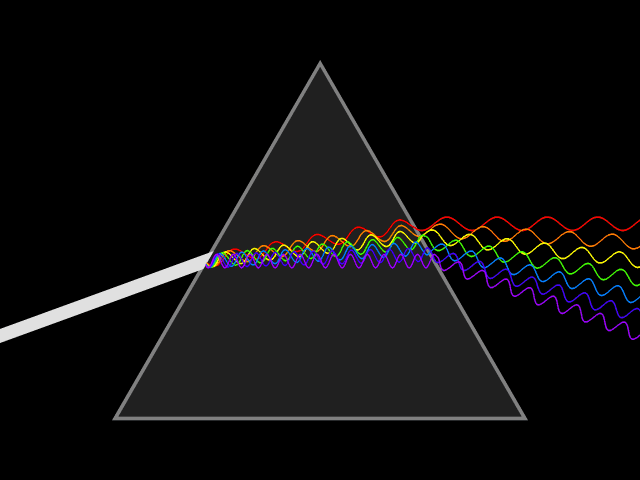
\includegraphics[width=\textwidth]{ch06/figures/prism.png}
          \end{center}
          \caption{Light can be seen as a superposition of electromagnetic waves with different 
          amplitudes, phases, and frequencies. This can be easily visualized in practice with the 
          help of a prism or a diffraction grating.}
          \label{fig:prism_ex}
        \end{marginfigure}

  % Exercise 5
  \item This is a follow-up question to the previous one. Let's say that we had an arbitrary number 
  of solutions to the wave equation with different angular frequencies $\omega_n$ and phasors $E_n$:
        \begin{equation}
          \vec{E}(x,t) = \hat{y}\sum_n E_n e^{i (\omega_n/c) x} e^{i \omega_n t}
        \end{equation}
        Would this still satisfy the Maxwell's equations (i.e., the wave equation)? 
        Can electromagnetic waves be composed of a superposition of two-dimensional 
        plane waves of different frequencies (wavelengths, or colors), which each 
        individually satisfy the wave equation?

  % Exercise 6
  \item Copy the example program in Listing \ref{lst:mixing_ex} that performs mixing and run it. 
        The example shows how to shift a complex exponential signal with a certain frequency to another frequency.
        Modify the script in such a way that the resulting complex exponential 
        signal \verb|z_shifted| has a frequency of 42 Hz. Use the plot to verify that the 
        frequency of the signal is approximately 42 Hz.

  % Exercise 7
  \item Go back to the guitar amplifier program
        \texttt{003\_guitar/amplifier.py}. We will now add one more
        effect. We'll modify the program so that it implements a modulation effect.

        \begin{itemize}
          % Exercise 7a)
          \item[a)] Multiply the clean guitar signal with a 5 Hz sinusoidal signal. Plot the signal.
\begin{lstlisting}[language=Python]
# Multiply with sinusoid.
x_mod = x*np.cos(2.0*np.pi*time_vec*5.0)
# Plot result.
plt.plot(time_vec, x_mod)
plt.show()
\end{lstlisting}
          % Exercise 7b)
          \item[b)] Write the output into an audio file and play the
                result. What does the output sound like?
\begin{lstlisting}[language=Python]
# Write compressed output to wav file. 
sio.write("guitar_leslie.wav", sample_rate, x_mod)
\end{lstlisting}

          % Exercise 7c)
          \item[c)] Change the frequency of the modulating sinusoid from 5 Hz to 2.5 Hz. 
          Predict what the audio will sound like. Play the resulting audio to confirm your hypothesis.

        \end{itemize}
        If you want to reflect on what is going on here, think of the original
        audio signal $x(t)$ as something that consists of a sum of sinusoidal
        signal components\sidenote{We'll introduce this properly later on}
        \begin{equation}
          x(t) = \sum_{n} A_n \cos(\omega_n t + \phi_n)
        \end{equation}
        When multiplying this signal with a sinusoidal signal of frequency $\omega$, we get a modulated audio signal $y(t)$:
        \begin{align}
          y(t) & = x(t) \cos(\omega t)                                                 \\
          y(t) & = \left[\sum_{n} A_n \cos(\omega_n t + \phi_n)\right] \cos(\omega t).
        \end{align}
        Each spectral component of a signal $x(t)$ gets the same treatment as you already investigated in Exercise 3.

\end{enumerate}